\chapter{Garden Gem} % Main chapter title

\label{Chapter:OurContribution}

Plentiful, healthy, economic and safe food for the entire planet is a topic to be held in our minds for the following years. Food safety and security are the main challenges to be discussed along with the confrontations against climatic change. At least 55\% of the world’s population already lives in urban areas, and this number is expected to rise to 65\% by 2050. (FAO, 2019) Nearly 80\% of all food produced is consumed in these urban areas and, according to information of the Food and Agriculture Organization of the United Nations, 60\% of irrigated and 35\% of rainfed croplands are within a 20 km radius of urban agglomerations. (FAO, 2019) Additionally, almost one third of all food produced for humans is lost into waste that comprises more than 50\% of all municipal waste. (FAO, 2019) Finally, it is important to point out that in low-income countries, food expenditures can take up to two thirds of the total household. (FAO, 2019) Food policies require training citizens about new lifestyles. The training purpose is to incentivize awareness to address sustainable food safety and security. (Sandrini, 2014)
The lifestyle of human kind shall be amended, particularly in regards of our food supply chain, from the farming, distribution to the end consumer. Through food education, the system players (consumers and producers) are trained. A new lifestyle will also have an environmental impact related to transportation and distribution. (Sandrini, 2014)

It is important to conserve farming land, especially in areas already subject to strong urbanization. GardenGem’s purpose is to be a tool for urban gardeners, researchers and citizens for food education and urban agriculture.

\section{Impact on the Economic Dimension}

Urban gardening has been part of the human economic activities since the emergence of cites as the urban phenomena developed. (Calvet-Mir, L., \& March, H., 2019) A study carried out by Calvet-Mir, L. \& March, H. established the importance of urban gardening as a response to financial crisis and their strong correlation to community resilience against war and other adversities. Populations of growing poverty rates in cities are also impacted by the development of urban gardens. Self-production or self-sufficiency of food are directly related to food security during economic crisis and shortages. Helping build self-sufficient cities improves the health and quality of food and rises awareness around local produce food sovereignty.

As detailed in Section \ref{sec:economicDim}, GardenGem takes this perspective into account, trying to aim towards an economically sustainable activity that can provide better food prices and optimal operational costs to any user of the application.

\section{Impact on the Social Dimension}

Urban gardening comes as a response to changing social and political circumstances. There have been numerous initiatives to promote their practice during conflicts and economic crisis to tackle food distribution problems during specific historical moments. These factors have an important effect shaping the form, function and culture of urban gardens and their members \cite{Calvet-Mir2019}. Since the last century, we have witnessed a growing institutional recognition of urban gardening, through national and local legislation in many countries, including Mexico.

Urban gardening portrays emancipatory and alternative views about the urban development and social relations. There is evidence of urban gardens being used to protest against political corruption, empowering the people and appealing to citizen responsibility to overcome any crisis \cite{Certoma2015}. Social entrepreneurship and social innovation are strongly related to urban gardening since it is subject of continuous improvement mainly due to the huge positive impact it has in people’s lives. It has been demonstrated that urban gardens have the effect of strengthening community ties, enabling intercultural exchanges, facilitating community building as and enhancing social cohesion where the garden is located \cite{Calvet-Mir2019}.

The GardenGem team is making research on these aspects to develop the right campaign for the encouragement of urban agriculture. We are working to find the correct approach towards people and government for incentivization and support. Section \ref{sec:socialDim} lists the social impact that Garden Gem is targeting.


\section{Impact on the Environmental Dimension}

Human beings have been altering their environment since the beginning of their existence; in fact, this specific trait is the most concluding evidence of human presence in any place or time. Urban planning is the practice of spatial arrangement of urban areas \cite{Certoma2015}. These arrangements unequivocally have an impact on the environment, thus the planification of cities must always consider alternatives for the best land distribution to allow human development without strangling itself by damaging its resources. Urban agriculture enhances the diversity and distribution of food and non-food products through processes that reuse human and material resources. This has a positive impact in and around the urban area supplying products and services to the same area in return \cite{Broadway2009}.

We want to prepare people with tools that empower them to take their environmental impact on their hands and start acting positively in the right direction. GardenGem is meant to improve the caring of the environment in a sustainable and practical way, by impacting the processes in Section \ref{sec:environmentalDim}.

\section{Garden Gem Objectives}

GardenGem is a mobile application that will help urban gardeners by assisting them in the correct development and maintenance of their urban gardens. Garden Gem’s will provide the information required to find compatible food plants with similar care and know the number of plants that can be placed within a given land area. Additionally, it will offer an in-app store to facilitate the purchase of materials and supplies for the optimal development of their urban garden. Further into the future, the app will feature a community intercommunication between urban gardeners to allow sharing and trading. The compatibility with other technologies as the Food Computer from the Open Agriculture Iniciative from the MIT will make this application even more useful for the automation of urban garden production.

Economical goal: To enable the average citizen, and local community to grow vegetables locally in order to save money and create a possible source of income. 

Social goal: To promote social integration and combat poverty by the creation of urban garden communities based on participation.

Environmental goal: To enhance the diversity and distribution of food products through processes that reuse resources in a sustainable and local way.

\subsection{Monetization}

The monetization of this product will be based in the in-app store where users and suppliers will receive small fees for each buy. One product that is expected to become a popular purchase is the kit for the construction of a Food Computer, since all the manuals and designs are openly available in the Open Agriculture Initiative. These fees will be the main source of income in the beginning. Once the community functionality is ready, trading fees between gardeners and direct consumers or distributors will support the application and its growth.

\section{Garden Gem Results}
\subsection{Development of the mobile application}

\begin{figure}[th]
\centering
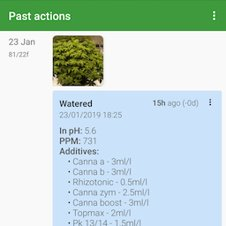
\includegraphics[width=0.45\textwidth]{./Figures/app1.png}
\decoRule
\caption[Record of the actions done to a given plant]{Record of the actions done to a given plant}
\label{fig:app1}
\end{figure}

\begin{figure}[th]
\centering
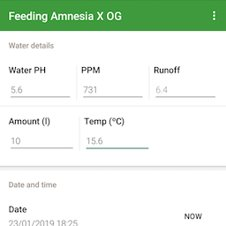
\includegraphics[width=0.45\textwidth]{./Figures/app2.png}
\decoRule
\caption[Feeding Amnesia X OG, characteristics]{Feeding Amnesia X OG, characteristics}
\label{fig:app2}
\end{figure}

\begin{figure}[th]
\centering
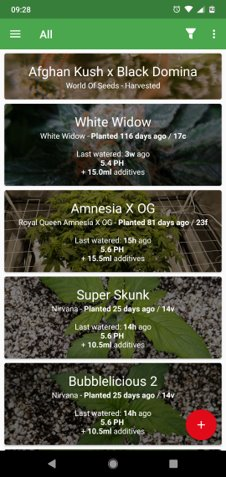
\includegraphics[width=0.45\textwidth]{./Figures/app3.png}
\decoRule
\caption[All plants]{All plants}
\label{fig:app3}
\end{figure}

The application can record data about growing plants in order to monitor the growing conditions and make the plants grow better by identify potential issues during the growing process. The application is also concentrating in the three pillars of sustainability focusing on its impact in the improvement of life standards for any user of our application according to the economic, environmental and social perspectives that were previously described in this project.

Figures \ref{fig:app1}, \ref{fig:app2} and \ref{fig:app3} show the final application running on an android device. In Figure 1 the actions that have been already done to the plant are recorded and showed. Figure 2 shows the proper characteristics needed for feeding Amnesia X OG. Finally, figure 3 shows all the current plants that are intended to growth in the best possible way.

According to the surveys performed to people from multiple backgrounds, the application received an approval rate of above 95\%. More than 60\% of the people who participated on the survey were already considering urban gardens before checking our app, and more than 90\% thought it would be useful. The complete results of this survey are presented in the annex section of this document.

%\begin{figure}[th]
%\centering
%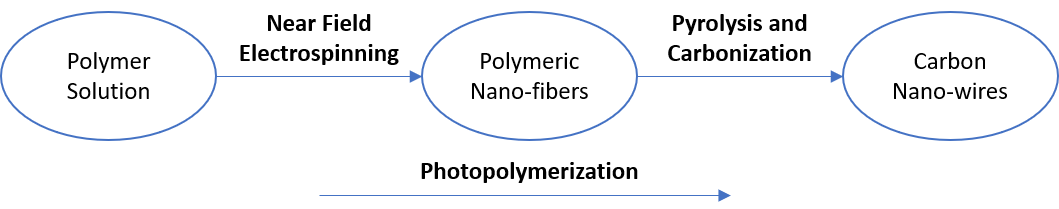
\includegraphics[width=0.95\textwidth]{./Figures/FabricationProcess.png}
%\decoRule
%\caption[Carbon Nano-wires Fabrication Process]{Fabrication process of carbon nano-wires to achieve through the proposed dissertation.}
%\label{fig:fabricationFlowChart}
%\end{figure}

%\begin{equation}
%\left(\tau _t^e-\frac{\tau _n^e \text{dr}}{\text{dz}}\right) 2 \pi  r+\frac{d \left(\pi  r^2
%   \left(\tau _{\text{zz}}-p\right)\right)}{\text{dz}}+\frac{\gamma  \text{dr} 2 \pi  r}{r
%   \text{dz}}+\rho  g \pi  r^2=\frac{d \left(\rho  \pi  r^2 v^2\right)}{\text{dz}}
%\label{eq:linearMomentum}
%\end{equation}